\documentclass[a4paper,10pt]{article}
%\usepackage[latin1]{inputenc} % Paquetes de idioma
\usepackage[utf8]{inputenc} % Paquetes de idioma (Este encoding toma acentos :) )
\usepackage[spanish]{babel} % Paquetes de idioma
\usepackage{graphicx} % Paquete para ingresar gráficos
\usepackage{grffile}
\usepackage{hyperref}
\usepackage{fancybox}
\usepackage{amsmath}
\usepackage{amsfonts}
\usepackage{listings}
\usepackage{float}
% Paquetes de macros de Circuitos
%\usepackage{pstricks}
\usepackage{tikz}
\usepackage{pdfpages}

% Encabezado y Pié de página
\usepackage{fancyhdr} % Paquete para encabezados y pie de página
\pagestyle{fancy} % Sin esta línea no se imprimiría el encabezado en todas las páginas

\fancyhf{} %  Borra el encabezado anterior (Por defecto escribe el títutlo de la sección en la que se encuentra la hoja
\setlength{\headheight}{22.55pt}
\fancyhead[L]{
	{\textsf{Facultad de Ingenier\'ia $-$ Universidad de Buenos Aires \\ 66.44 Instrumentos Electrónicos}}
}
%\addtocounter{page}{5}
\fancyhead[R]{\thepage}

\renewcommand{\footrulewidth}{0.4pt} % Ajusta el tamaño de las líneas separadoras en el pié de página
\renewcommand{\headrulewidth}{0.4pt} % Ajusta el tamaño de las líneas separadoras en el encabezado

\fancyfoot[L]{
	{\textsf{Trabajo Pr\'actico N$^{\circ}4$}: Mediciones de impedancias} \\
	{\textsf{Integrantes: Eduardo Sanchez, Francisco Soler}}
	}
		

% Carátula del Trabajo
\title{ \author{} % Lo pongo para que el warning no moleste :p
\setlength{\unitlength}{1cm} %  Especifica la unidad de trabajo
\thispagestyle{empty}

\begin{picture}(18,0)
\put(0,0){
\includegraphics[width=1.5cm, height=3cm]{Logo1.png}}

\put(10.5,0){
\includegraphics[width=3cm, height=3cm]{Logo2.png}}

\end{picture}
\\[1.5cm]
\begin{center}
	\textbf{{\Huge Facultad de Ingenier\'ia \\ Universidad de Buenos Aires}}\\[2cm]
	{66.44 Instrumentos Electrónicos}\\[0.5cm]
	{Trabajo Pr\'actico N$^{\circ}3$: Mediciones de impedancias}\\[2.5cm]
\end{center}

\begin{flushleft}
	\textbf{Integrantes:} \\[1cm]

	\begin{tabular}{|c|c|c|}
		\hline
		\textbf{\normalsize Padr\'on} & \textbf{\normalsize Nombre} & \textbf{\normalsize Email} \\
		\hline
		\normalsize 92903 & \normalsize Sanchez, Eduardo Hugo & \normalsize hugo\_044@hotmail.com \\
		\hline
		\normalsize 91227 & \normalsize Soler, Jos\'e Francisco & \normalsize francisco.\_tw@hotmail.com \\
		\hline
		\normalsize xxx & \normalsize Wawrynczak, Claudio  & \normalsize claudiozak@gmail.com \\
		\hline
	\end{tabular}
\end{flushleft}
\date{} % Hace que no se imprima la fecha en la cual se compilo el .tex
 }

\begin{document}
	\maketitle % Hace que el título anterior sea el principal del documento
	\newpage

	\tableofcontents % Esta línea genera un indice a partir de las secciones y
					 % subsecciones creadas en el documento
	\newpage


	\section{Objetivo}
	
	\indent	El objetivo del presente trabajo práctico es determinar el 
	comportamiento de 3 tipos de puntas de medición, de tensión 
	con alta/baja impedancia de entrada, y de corriente.
	
	\newpage
	\section{Desarrollo}
		\indent Para llevar a cabo las mediciones, se utilizan los siguientes
		instrumentos:
		\begin{itemize}
			\item Un generador de señales con la capacidad de realizar un 
			barrido en frecuencias.
			\item Un osciloscopio con la capacidad de cambiar a alta o baja su
			impedancia de entrada.
			\item Las puntas de prueba.
			\item Un cable que interconecta el generador con el osciloscopio,
			el cual, se comporta como una línea de transmisión.
		\end{itemize}
				 
		\subsection{Punta de prueba X10}
		\indent Como se observa en la figura \ref{esq001} Se conecta el 
		generador de se\~nales a la entrada del CH1 del osciloscopio cuya 
		impedancia de entrada es de $50 \Omega$, al igual que la impedancia 
		caracter\'istica del cable coaxil que los conecta, de manera que 
		exista adaptaci\'on. Por otra parte se utiliza una punta x10 en el 
		channel 2 del osciloscopio conectada a un BCN T intercalado entre el 
		CH1 y el cable de conexión al generador. \\
		\indent Los modelos de los instrumentos utilizados son:
		
		\begin{itemize}
			\item Osciloscopio Rigol DS1302CA - 300MHz
			\item Punta RP3300 - 350 MHz
		\end{itemize}

		\begin{figure}[!htb]
			\centering
			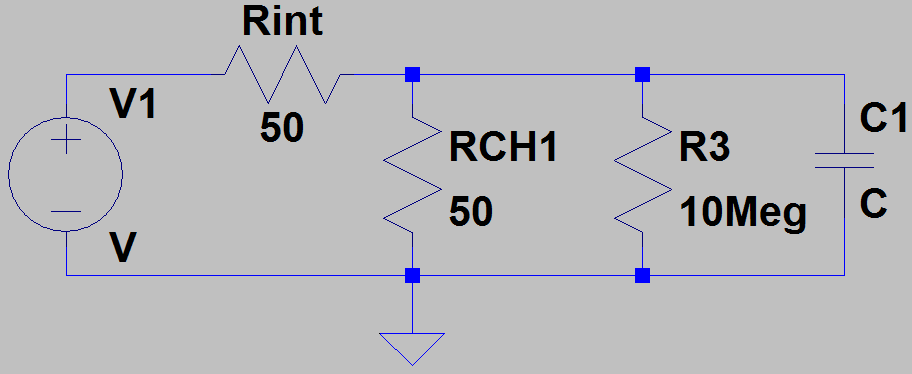
\includegraphics[width=8cm]
			{Esquematicos/EsqFrecCortePuntaX10.png}
			\caption{Circuito equivalente del banco de medición - punta x10} 
			\label{esq001}
		\end{figure}

		\indent El generador de se\~nales realiza un barrido de frecuencias de
		$1MHz$ a $400MHz$ en $10s$. En la Figura \ref{img001} se puede 
		observar las se\~nales en el CH1 cuando est\'a conectado al 
		generador de funciones (la cual se guarda como referencia) y cuando, 
		adem\'as, se carga el nodo del CH1 con la punta que se conecta al CH2.
		
		\begin{figure}[!htb]
			\centering
			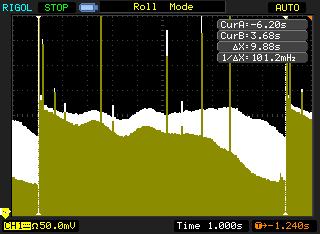
\includegraphics[width=8cm]
			{Imagenes/Mediciones instrumentos/NewFile1.png}
			\caption{Se\~nales medidas con el CH1 cuando est\'a conectado al 
			generador de se\~ales (en blanco) y cu\'ando se carga con la punta
			X10 (en verde).} \label{img001}
		\end{figure}
			
		\indent Como era de esperar al cargar el nodo con la punta X10, el 
		ancho de banda disminuye considerablemente. Aproximadamente la 
		frecuencia de corte observada en la Figura es $$f_{-3dB}=245MHz$$

		\indent Como se puede observar, hay diferentes amplitudes de la señal
		medida a distintas frecuencias (menores a la frecuencia de corte), 
		esto podría ser debido al generador o al cambio del $Z_{in}$ del 
		osciloscopio. Para descartar la primera opción, se realizó la misma
		medición con otro osciloscopio y se observó que la respuesta no era la
		misma. Por ende, la respuesta no plana es debido a que el $Z_{in}$ del
		osciloscopio varía con la frecuencia.\\
		\indent A modo de Referencia, se midió la diferencia de tensión entre
		ambas señales en el CH1 a una frecuencia de $130MHz$:

		\begin{equation*}
			\Delta V_{db} = 20*log(6/5) = 1.58 db 
		\end{equation*}

		\indent En la Figura \ref{img000} se vizualizan las se\~nales que 
		toman CH1 y CH2. La se\~nal del CH1 es la misma que en el caso 
		anterior con el ancho de banda reducido por el efecto de carga 
		generado por la punta X10. Por otra parte la se\~nal del CH2 presenta
		un sobrepico en altas frecuencias en lugar de actuar como un sistema 
		de primer orden. Dicho sobrepico se debe a que el conector utilizado 
		como tierra en la punta se comporta como si fuese una inductancia, 
		para disminuirla lo más posible, se utilizó el terminal corto que
		se provee con la punta. \\
		
		\begin{figure}[!htb]
			\centering
			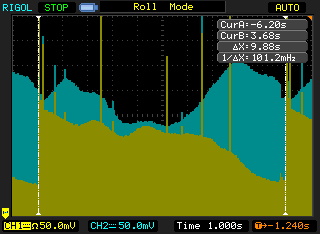
\includegraphics[width=8cm]
			{Imagenes/Mediciones instrumentos/NewFile0.png}
			\caption{Se\~nales del CH1 (en verde) y del canal CH2 (en celeste
			).} \label{img000}
		\end{figure}

		\indent Para calcular la inductancia equivalente que presenta el 
		terminal de tierra se utiliza la frecuencia de resonancia, la cual 
		es cuando $x_c = x_l$ y en el gráfico se observa con el sobrepico, el
		cual está a una frecuencia de $f = 245 MHz$. Tomando una capacidad 
		equivalente de la punta osciloscopio igual a $5pF$, la inductancia 
		del conector resulta:

		\begin{equation*}
			 L = \frac{1}{w^2*c} = 84 nHy 
		\end{equation*}

									
		\subsection{Punta de prueba X1}
		\indent Se realiza la misma experiencia que en el caso anterior, en la
		figura \ref{esq002} se observa el circuito equivalente del banco de 
		medición. El barrido de frecuencias es de $1MHz$ a $21MHz$ y la punta
		que se conecta al CH2 es X1. Dado que la punta X1 posee una 
		capacitancia equivalente mayor que la punta X10, es esperable que el 
		ancho de banda de la se\~nal se reduzca en mayor medida. \\

		\indent Los modelos de los instrumentos utilizados son:
		
		\begin{itemize}
			\item Osciloscopio: Rigol DS1302CA - 300MHz
			\item Punta: Rigol RP3300 - 350 MHz
		\end{itemize}

		\begin{figure}[!htb]
			\centering
			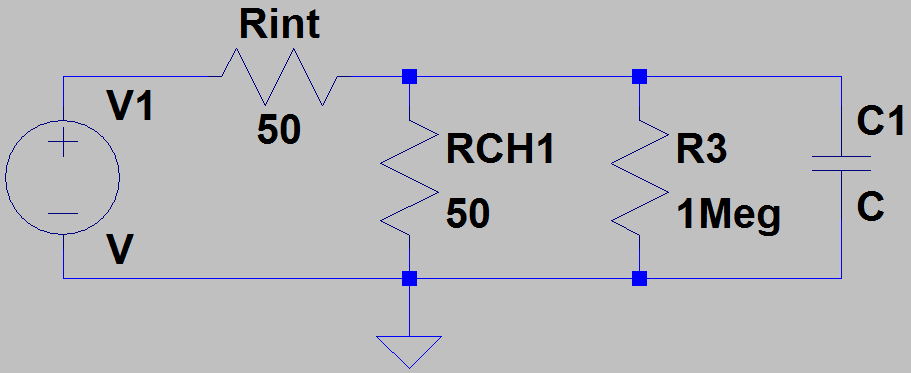
\includegraphics[width=8cm]
			{Esquematicos/EsqFrecCortePuntaX1.png}
			\caption{Circuito equivalente del banco de medición - punta X1} 
			\label{esq002}
		\end{figure}

		\indent En la Figura \ref{img003}, se pueden ver las se\~nales del CH1
		antes y despu\'es de cargarlo con la punta del CH2. A su vez se 
		aprecia que esta vez el osciloscopio presenta una respuesta mucho más
		plana en este rango de frecuencias ($z_{in}$ prácticamente no varía). \\
		\indent La atenuación en la señal medida por el CH1 luego de conectar
		el CH2 a la frecuencia de $11 MHz$ es de 
		$$ 20\cdot \log_{10}10/9 = 0.92db $$
		
		\begin{figure}[!htb]
			\centering
			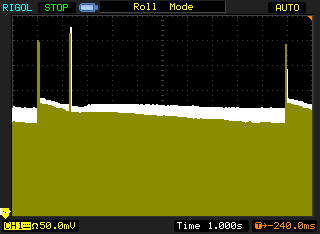
\includegraphics[width=8cm]
			{Imagenes/Mediciones instrumentos/NewFile4.png}
			\caption{Se\~nales del CH1 cuando est\'a conectada al generador 
			(en blanco) y cuando se carga con la punta X1(en verde).} 
			\label{img003}
		\end{figure}
		
		\indent Por otra parte en la Figura \ref{img002}, se pueden ver las 
		se\~nales que proviene del CH1 y el CH2. \\
		\indent La frecuencia de corte observada en la Figura es 
		$$f_{-3dB}=9MHz$$
		\indent La medición muestra que la punta x1 tiene un mayor ancho de 
		banda que la que indica el fabricante en la hoja de datos
		$BW = 8 MHz$
		\begin{figure}[!htb]
			\centering
			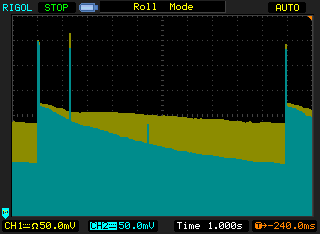
\includegraphics[width=8cm]
			{Imagenes/Mediciones instrumentos/NewFile3.png}
			\caption{Se\~nales del CH1 (en verde) y del canal CH2 (en celeste)
			.} \label{img002}
		\end{figure}						
	
		\indent A modo de comparación se midió a $5 MHz$ la diferencia en 
		decibeles entre el CH1 Y CH2 $$dif = 20*\log_{100/85}  = 1.41db $$

		\subsection{Punta de prueba de corriente}
		\indent En esta secci\'on se comparan los anchos de banda de puntas de
		corriente de dos fabricantes, Agilent$_{\textregistered}$  y 
		Tektronix$_{\textregistered} )$. \\
		\indent El procedimiento es similar al realizado en las experiencias 
		previas. Se utiliza un generador de se\~nales que barre frecuencias 
		desde $300KHz$ a $30MHz$ en un tiempo aproximado de $10s$, la 
		corriente que circula por el coaxil que se conecta al generador es 
		sensada por las puntas de corriente (2 por cada fabricante). En la 
		Figura \ref{img004} y \ref{img005}, se muestran los gr\'aficos 
		obtenidos para las puntas de Agilent$_{\textregistered}$. Los anchos de
		banda obtenidos de los gr\'aficos, son respectivamente 
		$$f_{-3dB}=15.6MHz$$ y $$f_{-3dB}=9.5MHz$$
	
		\indent Los modelos de los instrumentos utilizados son:
		
		\begin{itemize}
			\item Punta: Agilent 456A - (100Hz - 8MHz)
			\item Punta: Tektronix 6021 - (12Hz - 28MHz) 
		\end{itemize}

		\begin{figure}[!htb]
			\centering
			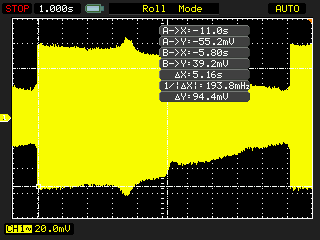
\includegraphics[width=8cm]
			{Imagenes/Mediciones instrumentos/NewFile5.png}
			\caption{Barrido en frecuencia para una punta de 
			Agilent$_{\textregistered}$.} \label{img004}
		\end{figure}
		
		\begin{figure}[!htb]
			\centering
			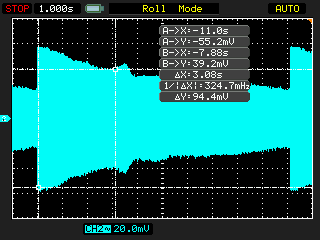
\includegraphics[width=8cm]
			{Imagenes/Mediciones instrumentos/NewFile6.png}
			\caption{Barrido en frecuencia para una punta de 
			Agilent$_{\textregistered}$.} \label{img005}
		\end{figure}				
		
		\indent Por otra parte, dado que las puntas de corriente de 
		Tektronix$_{\textregistered} )$ tienen menor ancho de banda se 
		modific\'o el rango de barrido del generador a $300kHz$ a $10MHz$.En 
		las Figuras \ref{img006} y \ref{img007}, se muestran los gr\'aficos 
		obtenidos. De ellos se puede calcular el ancho de banda de cada punta
		$$f_{-3dB}=2.4MHz$$ y $$f_{-3dB}=1.9MHz$$
		\indent Las frecuencias de corte superior de las 4 puntas dieron muy 
		por debajo del ancho de banda determinado por el fabricante en la hoja 
		de datos.
		
		\begin{figure}[!htb]
			\centering
			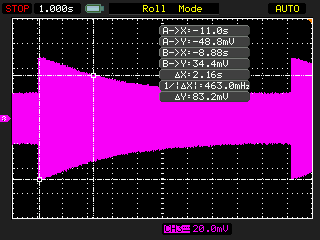
\includegraphics[width=8cm]
			{Imagenes/Mediciones instrumentos/NewFile7.png}
			\caption{Barrido en frecuencia para una punta de 
			Tektronix$_{\textregistered}$.} \label{img006}
		\end{figure}		
	
		\begin{figure}[!htb]
			\centering
			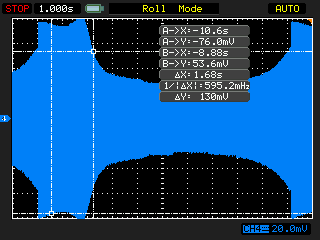
\includegraphics[width=8cm]
			{Imagenes/Mediciones instrumentos/NewFile8.png}
			\caption{Barrido en frecuencia para una punta de 
			Tektronix$_{\textregistered}$.} \label{img007}
		\end{figure}
	
		\indent Para determinar la frecuencia de corte inferior se utilizó el
		el banco de medición mostrado en la figura \ref{esq002}. En el CH1 del
		osciloscopio se dejó conectada la punta pasiva para tener como 
		referencia la tensión que hay en la resistencia. \\
		\indent Como las puntas de corriente son muy ruidosas, la medición no
		se realiza utilizando la detección de envolvente, el ruido eclipsa 
		completamente la medición. Para disminuir el ruido de alta frecuencia,
		se configuró el osciloscopio para que tenga un pasa bajo a $20 MHz$\\
%
%		\begin{figure}[!htb]
%			\centering
%			\includegraphics[width=8cm]
%	 		{Esquematicos/esqFreqCorteInfPuntasCorriente.png}
%			\caption{Circuito equivalente del banco de medición freq inf 
%			puntas de corriente}
%		    \label{esq003}
%		\end{figure}

		\indent La figura \ref{img009} muestra:  \\
		\indent Izquierda: la tensión y corrietes medidas por las distintas 
		puntas a una frecuencia de $500Hz$. Como están dentro del ancho de 
		banda, la señal se la toma como referencia. \\
		\indent Centro: Muestra la frecuencia de corte inferior de la punta 
		Tektronix. \\
		\indent Derecha: Muestra la frecuencia de corte inferior de la punta 
		Agilent.\\
		\indent A modo de comparación, la tabla \ref{tab001} muestra los 
		resultados obtenidos comparándolos con el ancho de banda teórico.
		
		\begin{figure}[!htb]
			\centering
			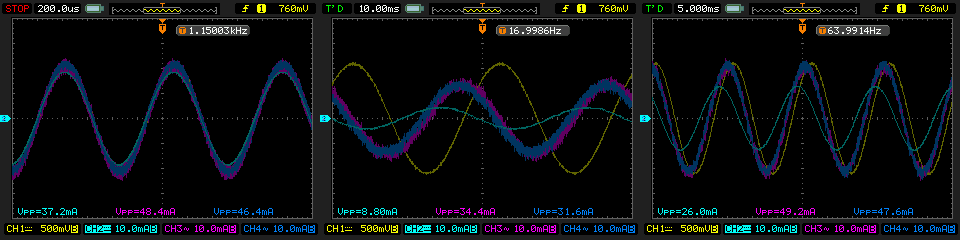
\includegraphics[width=12cm]
	 		{Imagenes/Mediciones instrumentos/frecCortePuntaCorriente.png}
			\caption{Izquierda: medición dentro del ancho de banda. Centro 
			frecuencia de corte de punta Tektronix. Derecha: frecuencia de corte
			inferior de punta Agilent}
		    \label{img009}
		\end{figure}
	
		\begin{table}
		\begin{tabular}{|c|c|c|c|c|}
			\hline
			 & \multicolumn{2}{|c|}{Teórico} & \multicolumn{2}{|c|}{medido} \\
			\hline
			& $Finf_{inferior}$ & $F_{superior}$ & $F_{inferior}$ & 
			$F_{superioro}$ \\
			\hline
			Agilent & 64Hz  & 2.4MHz  & 100 Hz & 8MHz \\
			\hline
			Tektronix & 17Hz & 15.6MHz  & 12Hz  & 28MHz \\
			\hline
		\end{tabular}
		\end{table}

		\newpage
		\subsection{Tiempo de crecimiento del conjunto punta-osciloscopio}
		
		\indent En esta secci\'on se mide el tiempo de crecimiento del 
		generador. \\
 		\indent Se conecta el generador de se\~nales a la entrada del CH1 del
		osciloscopio cuya impedancia de entrada es de $50 \Omega$, al igual 
		que la impedancia caracter\'istica del cable coaxil que los conecta, 
		de manera que exista adaptaci\'on. Por otra parte al CH2 del 
		osciloscopio se conecta una punta X10, la cual, sensa la tensi\'on a 
		la entrada del CH1. \\
		\indent En la Figura \ref{img008} muestra las se\~nales que
		reciben el CH1 (referencia) y el CH2. Se puede observar que el tiempo
		de crecimiento del CH2 es menor que el del CH1, esto se debe a que la
		punta posee una bobina de refuerzo de altas frecuencias, logrando así
		un tiempo de crecimiento menor al del circuito en medición.
		
		\begin{figure}[!htb]
			\centering
			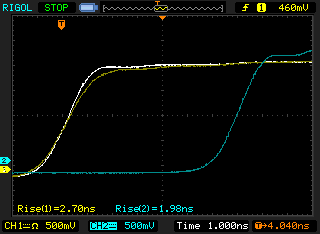
\includegraphics[width=8cm]
			{Imagenes/Mediciones instrumentos/NewFile10.png}
			\caption{Se\~nales del CH1 (en verde) y del canal CH2 (en celeste)
			} \label{img008}
		\end{figure}
		\indent El risetime medido es igual a $1,98 nSeg$, para obtener el 
		rise time de la punta, se puede utilizar la siguiente aproximación:
		$$Tr_{med}^2 = Tr_{gen}^2 + Tr_{punta}^2 + Tr_{osc}^2$$
		\indent Esta ecuación se la puede aplicar en caso de tener una cascada
		de cuadripolos, El problema es que los polos de los mismos tienen que 
		estar medianamente cerca, no lo suficiente, porque sino uno de los 
		términos (ej el despejado) de mucho menor a los demas rise time con 
		que se realizó la medición, llegando así a un error grosero. A su vez,
		tampoco pueden estar muy separados, porque de esta forma ni siquiera 
		entrarían en consideración. \\
		\indent En el caso de esta medición, los rise times obtenidos de las 
		hojas de datos de los fabricantes son los siguientes: 
		
		\begin{itemize}
			\item Generador: 1,7 nSeg  
			\item Osciloscopio: 1,2 nSeg
			\item punta: 900 pSeg
		\end{itemize}
		\indent Dado que los rise time del generador y del osciloscopio son 
		ambos mayores al de la punta y próximos entre si, no tiene sentido 
		realizar el cálculo. \\
		\indent Para expresar el resultado de la medición con incertidumbres,
		se obtienen los datos del osciloscopio que posee la siguiente 
		incertidumbre en el canal horizontal en modo tiempo equivalente
		$$ \frac{1}{50GSa} + 50ppm * reading + 0.6 ns$$
		$$ Tr_{med} = 1.98 nSeg \pm 0.62 nSeg$$

	\newpage
	\section{Conclusiones}
	\indent Existe una innumerable cantidad de puntas, hay que tener en cuenta
	que clase de medición se desea realizar, que características posee el 
	circuito a medir y cuales son las características del osciloscopio a la 
	hora de elegir la punta a utilizar. \\
	\indent En una primera aproximación se puede llegar a pensar que una punta
	de alta impedancia es mejor que una de baja impedancia, pero a la hora de
	realizar una medición en alta frecuencia, se da el caso que la segunda 
	posee una impedancia de entrada mayor que la primera.\\
	\indent A la hora de hacer una medición de alguna magnitud en particular,
	hay que tomar extrema precaución que dicha magnitud sea la dominante en el
	circuito completo, ejemplo: para medición del rise time de una punta, es 
	necesario que el rise time del osciloscopio como del generador sea mucho 
	menor. 
	
	\newpage
	\section{Anexo}
	\subsection{Punta pasiva}
	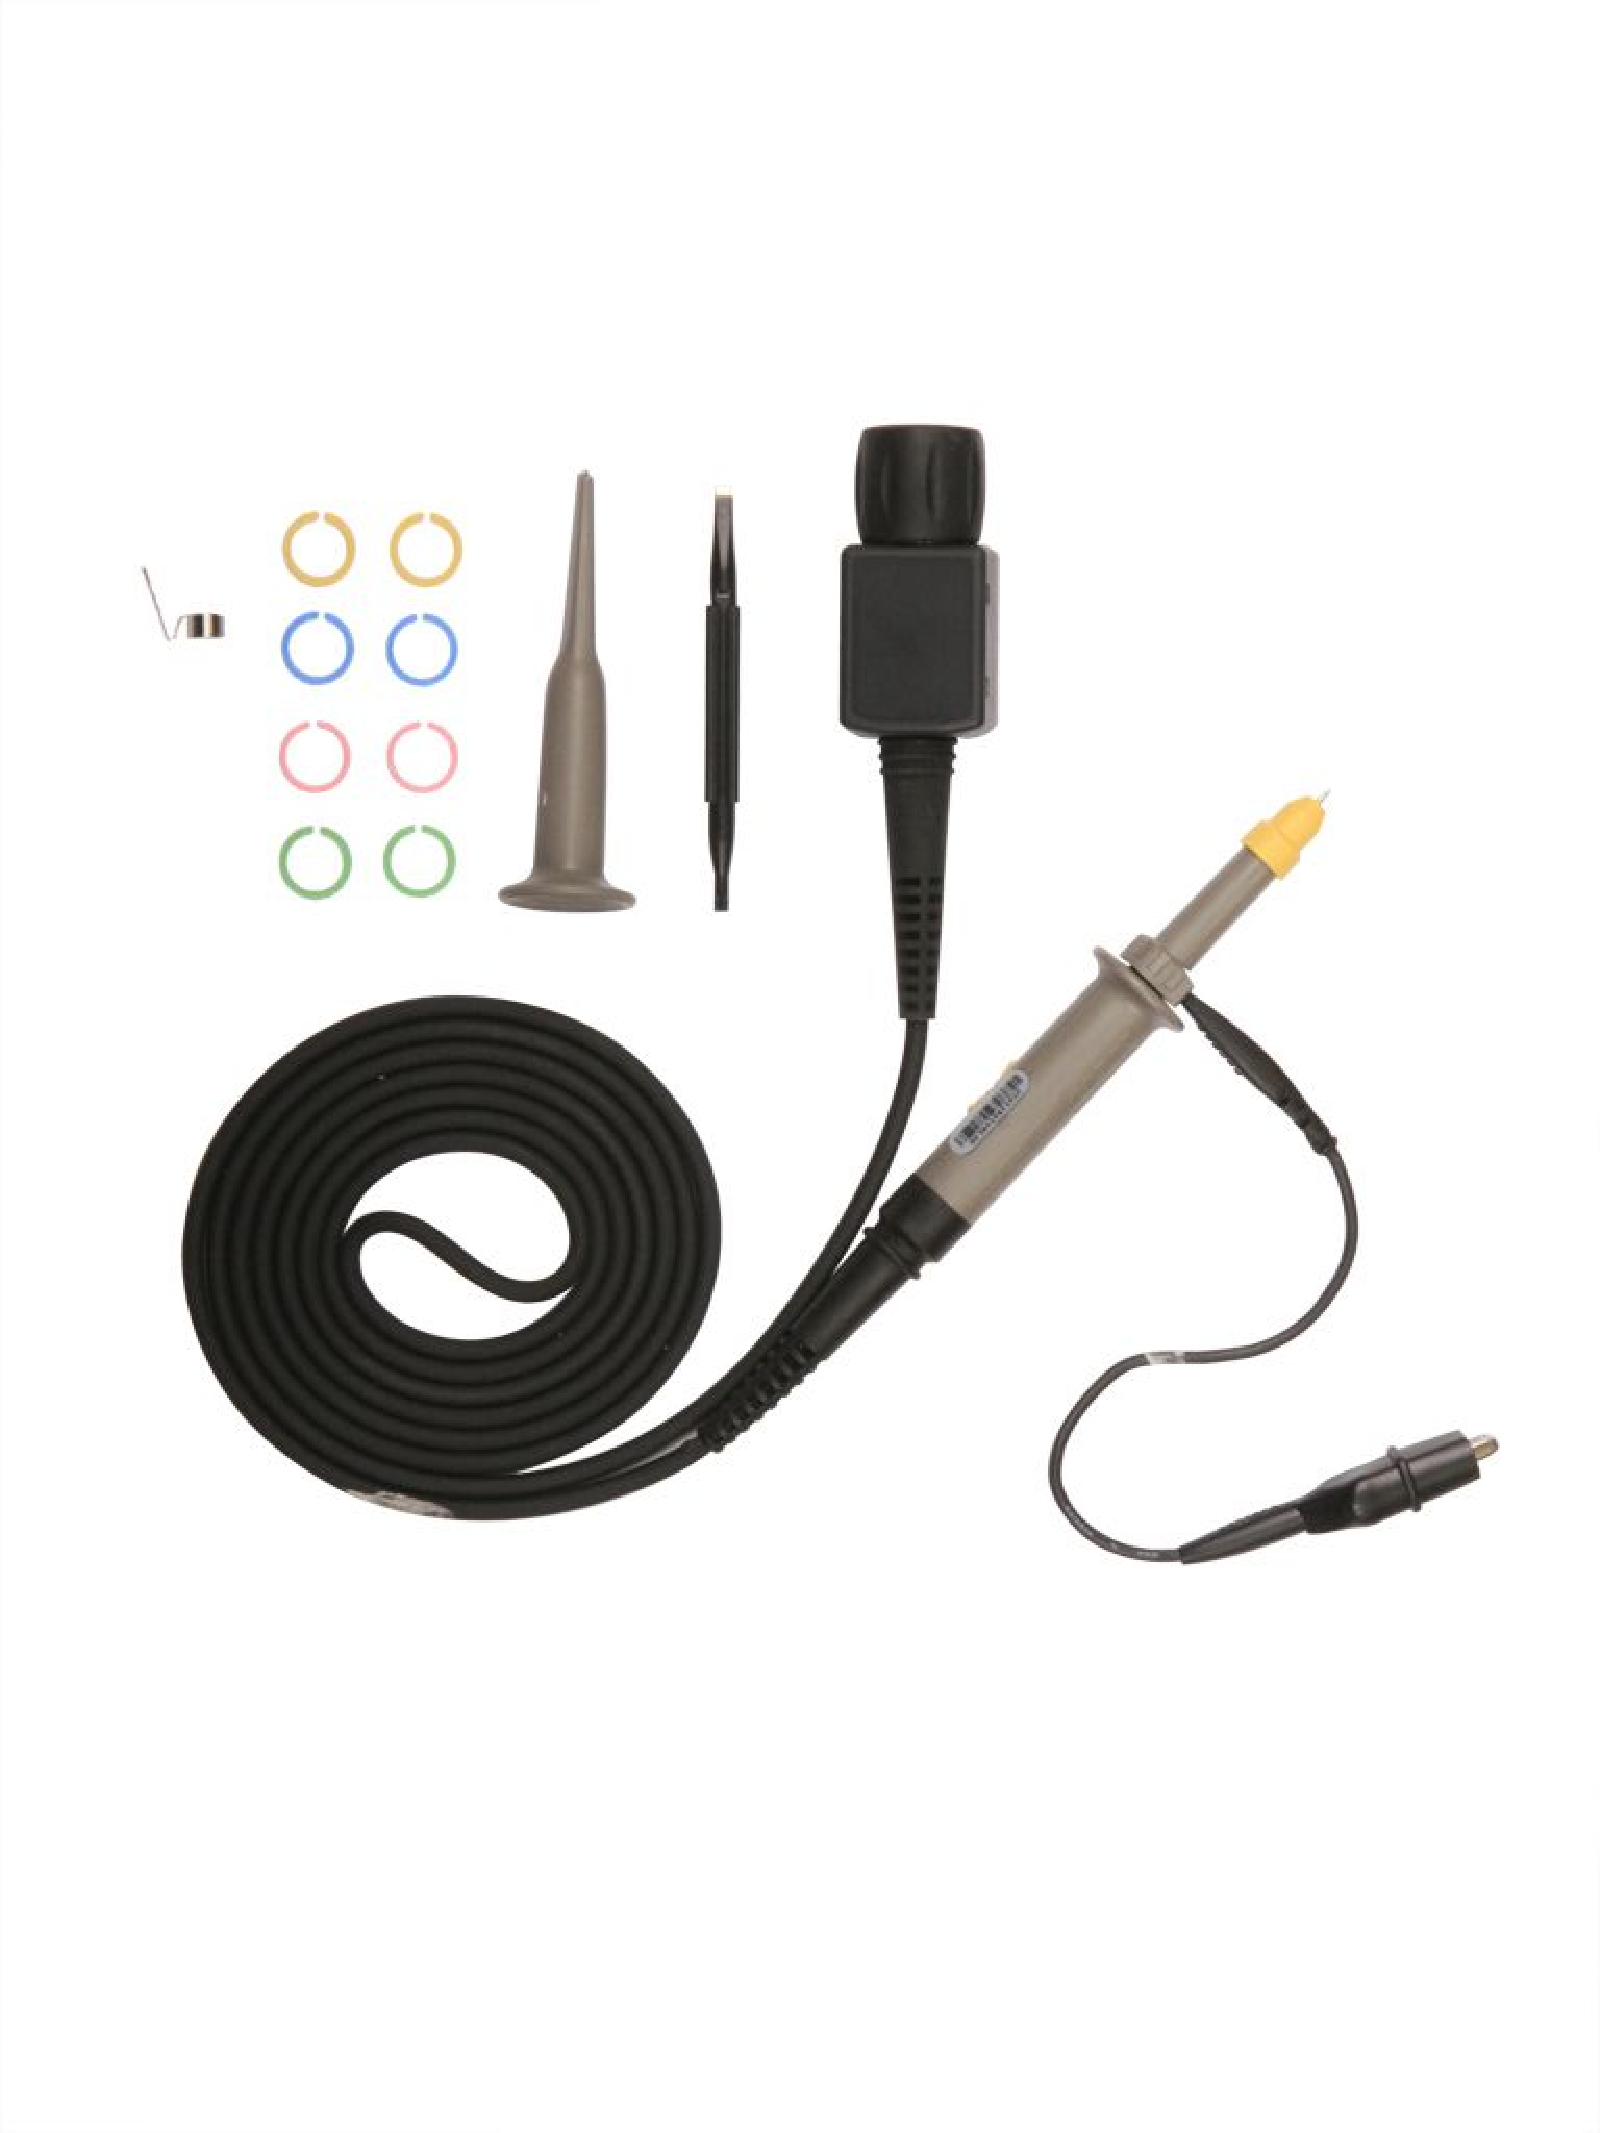
\includepdf[pages={-}]{hojas de datos/RP3300 guide.pdf}

	\newpage
	\subsection{Puntas de corriente}
	\includepdf[pages={-}]{hojas de datos/tek P6021 type 134.pdf}
	
\includepdf[pages={-}]{hojas de datos/HP-456A-Manual.pdf}
	
	\newpage
	\subsection{Osciloscopio}
	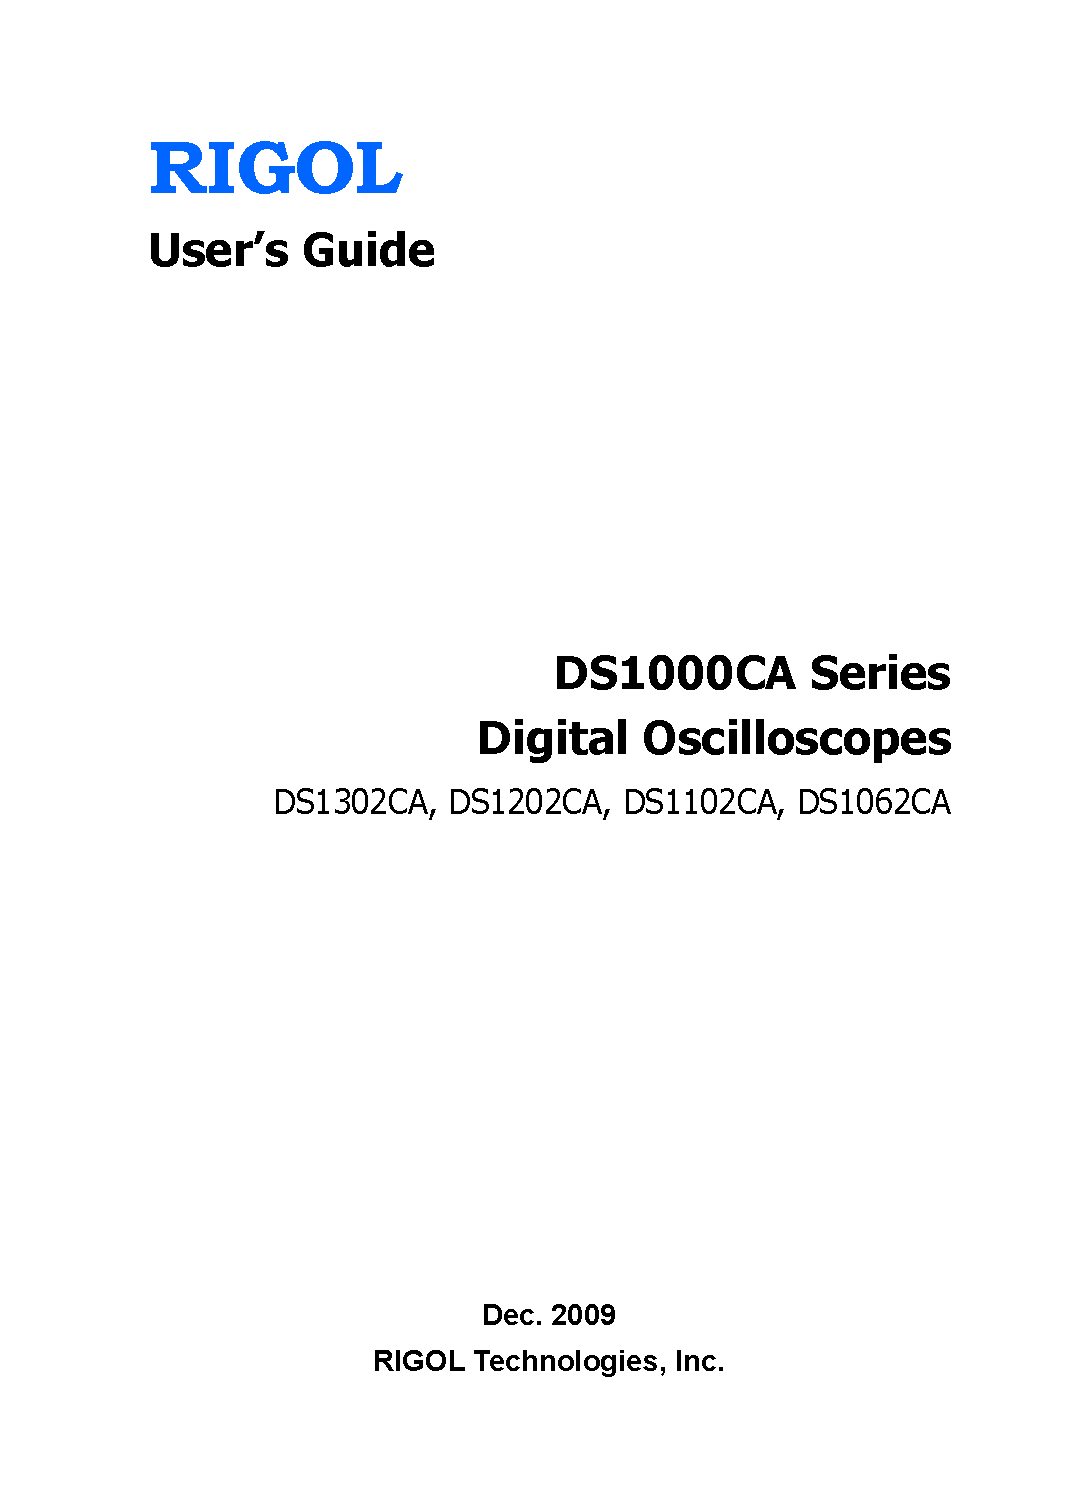
\includepdf[pages={-}]{hojas de datos/Rigol DS1302CA User's Guide.pdf}

\end{document}

